% Created by tikzDevice version 0.10.1 on 2017-10-12 17:15:30
% !TEX encoding = UTF-8 Unicode
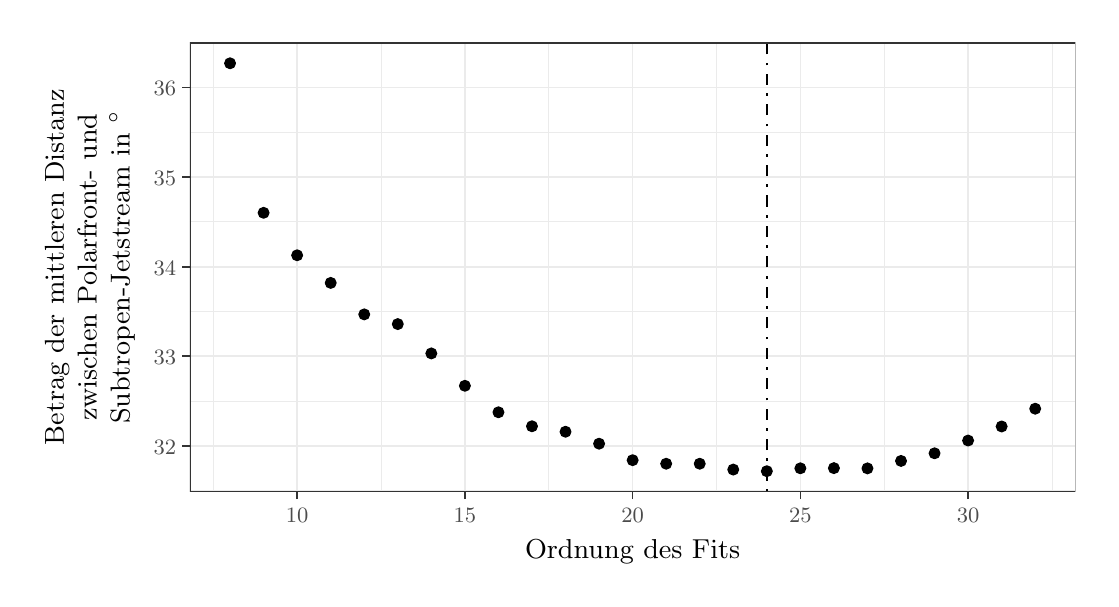
\begin{tikzpicture}[font=\small,x=1pt,y=1pt]
\definecolor{fillColor}{RGB}{255,255,255}
\path[use as bounding box,fill=fillColor,fill opacity=0.00] (0,0) rectangle (384.11,199.17);
\begin{scope}
\path[clip] (  0.00,  0.00) rectangle (384.11,199.17);
\definecolor{drawColor}{RGB}{255,255,255}
\definecolor{fillColor}{RGB}{255,255,255}

\path[draw=drawColor,line width= 0.6pt,line join=round,line cap=round,fill=fillColor] (  0.00,  0.00) rectangle (384.11,199.17);
\end{scope}
\begin{scope}
\path[clip] ( 58.58, 31.53) rectangle (378.61,193.67);
\definecolor{fillColor}{RGB}{255,255,255}

\path[fill=fillColor] ( 58.58, 31.53) rectangle (378.61,193.67);
\definecolor{drawColor}{gray}{0.92}

\path[draw=drawColor,line width= 0.3pt,line join=round] ( 58.58, 31.84) --
	(378.61, 31.84);

\path[draw=drawColor,line width= 0.3pt,line join=round] ( 58.58, 64.22) --
	(378.61, 64.22);

\path[draw=drawColor,line width= 0.3pt,line join=round] ( 58.58, 96.60) --
	(378.61, 96.60);

\path[draw=drawColor,line width= 0.3pt,line join=round] ( 58.58,128.98) --
	(378.61,128.98);

\path[draw=drawColor,line width= 0.3pt,line join=round] ( 58.58,161.35) --
	(378.61,161.35);

\path[draw=drawColor,line width= 0.3pt,line join=round] ( 67.07, 31.53) --
	( 67.07,193.67);

\path[draw=drawColor,line width= 0.3pt,line join=round] (127.68, 31.53) --
	(127.68,193.67);

\path[draw=drawColor,line width= 0.3pt,line join=round] (188.29, 31.53) --
	(188.29,193.67);

\path[draw=drawColor,line width= 0.3pt,line join=round] (248.90, 31.53) --
	(248.90,193.67);

\path[draw=drawColor,line width= 0.3pt,line join=round] (309.52, 31.53) --
	(309.52,193.67);

\path[draw=drawColor,line width= 0.3pt,line join=round] (370.13, 31.53) --
	(370.13,193.67);

\path[draw=drawColor,line width= 0.6pt,line join=round] ( 58.58, 48.03) --
	(378.61, 48.03);

\path[draw=drawColor,line width= 0.6pt,line join=round] ( 58.58, 80.41) --
	(378.61, 80.41);

\path[draw=drawColor,line width= 0.6pt,line join=round] ( 58.58,112.79) --
	(378.61,112.79);

\path[draw=drawColor,line width= 0.6pt,line join=round] ( 58.58,145.17) --
	(378.61,145.17);

\path[draw=drawColor,line width= 0.6pt,line join=round] ( 58.58,177.54) --
	(378.61,177.54);

\path[draw=drawColor,line width= 0.6pt,line join=round] ( 97.37, 31.53) --
	( 97.37,193.67);

\path[draw=drawColor,line width= 0.6pt,line join=round] (157.99, 31.53) --
	(157.99,193.67);

\path[draw=drawColor,line width= 0.6pt,line join=round] (218.60, 31.53) --
	(218.60,193.67);

\path[draw=drawColor,line width= 0.6pt,line join=round] (279.21, 31.53) --
	(279.21,193.67);

\path[draw=drawColor,line width= 0.6pt,line join=round] (339.82, 31.53) --
	(339.82,193.67);
\definecolor{drawColor}{RGB}{0,0,0}
\definecolor{fillColor}{RGB}{0,0,0}

\path[draw=drawColor,line width= 0.4pt,line join=round,line cap=round,fill=fillColor] ( 73.13,186.30) circle (  1.96);

\path[draw=drawColor,line width= 0.4pt,line join=round,line cap=round,fill=fillColor] ( 85.25,132.27) circle (  1.96);

\path[draw=drawColor,line width= 0.4pt,line join=round,line cap=round,fill=fillColor] ( 97.37,116.92) circle (  1.96);

\path[draw=drawColor,line width= 0.4pt,line join=round,line cap=round,fill=fillColor] (109.50,106.94) circle (  1.96);

\path[draw=drawColor,line width= 0.4pt,line join=round,line cap=round,fill=fillColor] (121.62, 95.57) circle (  1.96);

\path[draw=drawColor,line width= 0.4pt,line join=round,line cap=round,fill=fillColor] (133.74, 92.06) circle (  1.96);

\path[draw=drawColor,line width= 0.4pt,line join=round,line cap=round,fill=fillColor] (145.86, 81.46) circle (  1.96);

\path[draw=drawColor,line width= 0.4pt,line join=round,line cap=round,fill=fillColor] (157.99, 69.76) circle (  1.96);

\path[draw=drawColor,line width= 0.4pt,line join=round,line cap=round,fill=fillColor] (170.11, 60.19) circle (  1.96);

\path[draw=drawColor,line width= 0.4pt,line join=round,line cap=round,fill=fillColor] (182.23, 55.13) circle (  1.96);

\path[draw=drawColor,line width= 0.4pt,line join=round,line cap=round,fill=fillColor] (194.35, 53.16) circle (  1.96);

\path[draw=drawColor,line width= 0.4pt,line join=round,line cap=round,fill=fillColor] (206.48, 48.84) circle (  1.96);

\path[draw=drawColor,line width= 0.4pt,line join=round,line cap=round,fill=fillColor] (218.60, 42.88) circle (  1.96);

\path[draw=drawColor,line width= 0.4pt,line join=round,line cap=round,fill=fillColor] (230.72, 41.60) circle (  1.96);

\path[draw=drawColor,line width= 0.4pt,line join=round,line cap=round,fill=fillColor] (242.84, 41.60) circle (  1.96);

\path[draw=drawColor,line width= 0.4pt,line join=round,line cap=round,fill=fillColor] (254.96, 39.49) circle (  1.96);

\path[draw=drawColor,line width= 0.4pt,line join=round,line cap=round,fill=fillColor] (267.09, 38.90) circle (  1.96);

\path[draw=drawColor,line width= 0.4pt,line join=round,line cap=round,fill=fillColor] (279.21, 39.95) circle (  1.96);

\path[draw=drawColor,line width= 0.4pt,line join=round,line cap=round,fill=fillColor] (291.33, 40.01) circle (  1.96);

\path[draw=drawColor,line width= 0.4pt,line join=round,line cap=round,fill=fillColor] (303.45, 39.92) circle (  1.96);

\path[draw=drawColor,line width= 0.4pt,line join=round,line cap=round,fill=fillColor] (315.58, 42.61) circle (  1.96);

\path[draw=drawColor,line width= 0.4pt,line join=round,line cap=round,fill=fillColor] (327.70, 45.37) circle (  1.96);

\path[draw=drawColor,line width= 0.4pt,line join=round,line cap=round,fill=fillColor] (339.82, 49.98) circle (  1.96);

\path[draw=drawColor,line width= 0.4pt,line join=round,line cap=round,fill=fillColor] (351.94, 55.06) circle (  1.96);

\path[draw=drawColor,line width= 0.4pt,line join=round,line cap=round,fill=fillColor] (364.07, 61.48) circle (  1.96);

\path[draw=drawColor,line width= 0.6pt,dash pattern=on 1pt off 3pt on 4pt off 3pt ,line join=round] (267.09, 31.53) -- (267.09,193.67);
\definecolor{drawColor}{gray}{0.20}

\path[draw=drawColor,line width= 0.6pt,line join=round,line cap=round] ( 58.58, 31.53) rectangle (378.61,193.67);
\end{scope}
\begin{scope}
\path[clip] (  0.00,  0.00) rectangle (384.11,199.17);
\definecolor{drawColor}{gray}{0.30}

\node[text=drawColor,anchor=base east,inner sep=0pt, outer sep=0pt, scale=  0.88] at ( 53.63, 45.00) {32};

\node[text=drawColor,anchor=base east,inner sep=0pt, outer sep=0pt, scale=  0.88] at ( 53.63, 77.38) {33};

\node[text=drawColor,anchor=base east,inner sep=0pt, outer sep=0pt, scale=  0.88] at ( 53.63,109.76) {34};

\node[text=drawColor,anchor=base east,inner sep=0pt, outer sep=0pt, scale=  0.88] at ( 53.63,142.13) {35};

\node[text=drawColor,anchor=base east,inner sep=0pt, outer sep=0pt, scale=  0.88] at ( 53.63,174.51) {36};
\end{scope}
\begin{scope}
\path[clip] (  0.00,  0.00) rectangle (384.11,199.17);
\definecolor{drawColor}{gray}{0.20}

\path[draw=drawColor,line width= 0.6pt,line join=round] ( 55.83, 48.03) --
	( 58.58, 48.03);

\path[draw=drawColor,line width= 0.6pt,line join=round] ( 55.83, 80.41) --
	( 58.58, 80.41);

\path[draw=drawColor,line width= 0.6pt,line join=round] ( 55.83,112.79) --
	( 58.58,112.79);

\path[draw=drawColor,line width= 0.6pt,line join=round] ( 55.83,145.17) --
	( 58.58,145.17);

\path[draw=drawColor,line width= 0.6pt,line join=round] ( 55.83,177.54) --
	( 58.58,177.54);
\end{scope}
\begin{scope}
\path[clip] (  0.00,  0.00) rectangle (384.11,199.17);
\definecolor{drawColor}{gray}{0.20}

\path[draw=drawColor,line width= 0.6pt,line join=round] ( 97.37, 28.78) --
	( 97.37, 31.53);

\path[draw=drawColor,line width= 0.6pt,line join=round] (157.99, 28.78) --
	(157.99, 31.53);

\path[draw=drawColor,line width= 0.6pt,line join=round] (218.60, 28.78) --
	(218.60, 31.53);

\path[draw=drawColor,line width= 0.6pt,line join=round] (279.21, 28.78) --
	(279.21, 31.53);

\path[draw=drawColor,line width= 0.6pt,line join=round] (339.82, 28.78) --
	(339.82, 31.53);
\end{scope}
\begin{scope}
\path[clip] (  0.00,  0.00) rectangle (384.11,199.17);
\definecolor{drawColor}{gray}{0.30}

\node[text=drawColor,anchor=base,inner sep=0pt, outer sep=0pt, scale=  0.88] at ( 97.37, 20.52) {10};

\node[text=drawColor,anchor=base,inner sep=0pt, outer sep=0pt, scale=  0.88] at (157.99, 20.52) {15};

\node[text=drawColor,anchor=base,inner sep=0pt, outer sep=0pt, scale=  0.88] at (218.60, 20.52) {20};

\node[text=drawColor,anchor=base,inner sep=0pt, outer sep=0pt, scale=  0.88] at (279.21, 20.52) {25};

\node[text=drawColor,anchor=base,inner sep=0pt, outer sep=0pt, scale=  0.88] at (339.82, 20.52) {30};
\end{scope}
\begin{scope}
\path[clip] (  0.00,  0.00) rectangle (384.11,199.17);
\definecolor{drawColor}{RGB}{0,0,0}

\node[text=drawColor,anchor=base,inner sep=0pt, outer sep=0pt, scale=  1.10] at (218.60,  7.44) {Ordnung des Fits};
\end{scope}
\begin{scope}
\path[clip] (  0.00,  0.00) rectangle (384.11,199.17);
\definecolor{drawColor}{RGB}{0,0,0}

\node[text=drawColor,rotate= 90.00,anchor=base,inner sep=0pt, outer sep=0pt, scale=  1.10] at ( 13.08,112.60) {Betrag der mittleren Distanz };

\node[text=drawColor,rotate= 90.00,anchor=base,inner sep=0pt, outer sep=0pt, scale=  1.10] at ( 24.96,112.60) { zwischen Polarfront- und };

\node[text=drawColor,rotate= 90.00,anchor=base,inner sep=0pt, outer sep=0pt, scale=  1.10] at ( 36.84,112.60) { Subtropen-Jetstream in $^{\circ}$};
\end{scope}
\end{tikzpicture}
